% !TEX root = ../main.tex

\chapter{绪论}

\section{研究背景与意义}

全球卫星导航系统(Global Navigation Satellite System, GNSS)是由卫星星座向全球用户提供定位、导航和授时服务的空间系统。典型的GNSS包括美国的GPS、俄罗斯的GLONASS、欧洲的Galileo和中国的北斗卫星导航系统(BDS)等,它们通过卫星发射无线电导航信号,供用户接收机实时解算位置信息\cite{Li2015Precise}。在军用和民用领域,GNSS已成为时空信息获取的基础支撑,其功能涵盖从日常车辆导航、智能手机定位到航空航海、高精度测绘和授时同步等各个方面\cite{Jin2022A}。GNSS为全球经济发展和国家安全提供了关键支撑,被誉为现代社会的“时空基准”。

自20世纪70年代GPS首先部署以来,全球导航卫星系统得到了长足发展。GPS系统不断现代化,卫星更新换代并增加新信号频率,提高了服务精度和抗干扰能力;同时引入了如弹性功率(Flex Power)等新技术以增强军事信号的性能。俄罗斯的GLONASS完成恢复并实现全天候全球服务\cite{urlichich2011glonass};欧盟的Galileo系统于2019年底初步建成,提供全球服务\cite{fernandez2022galileo}。中国的北斗系统分三期建设,其中北斗三号(BDS--3)于2020年完成全球组网,采用了星间链路、新一代铷原子钟和被动氢原子钟等先进载荷设备与技术,显著提升了导航信号性能,其10天频率稳定度达到$10^{-–15}$量级,性能指标已经与GPS相当\cite{Yang2020Basic,Lu2020Global}。北斗系统创新融合了导航与通信能力,具备定位导航授时、星基增强、地基增强、精密单点定位、短报文通信和国际搜救等多种服务能力\cite{Yang2021Featured}。作为北斗三号系统特色服务之一,其播发B2b信号,向用户播发卫星轨道改正数、钟差改正数和码偏差等信息,可向中国及周边地区提供实时的精密单点定位(Precise Point Positioning, PPP) 服务\cite{Yang2022Principle}。

随着GNSS技术的发展,高精度定位方法逐步由依赖局部参考站的相对定位,向基于精密产品的绝对定位演进\cite{Elsheikh2023The,Hou2023Recent}。 实时动态差分定位(RTK)是较早实现工程化厘米级定位精度的技术之一\cite{Li2022Review}。该方法通过引入局域参考站,对流动站与参考站的观测值进行双差处理,有效消除了接收机与卫星钟差,并显著削弱轨道误差、对流层延迟及电离层延迟等空间相关误差,从而实现整周模糊度的快速固定,获得高精度定位结果\cite{Geng2011Towards}。然而,RTK的高精度建立在误差高度相关的基础之上,其定位性能随基线长度增加而明显下降,通常要求流动站与参考站之间的距离不超过20 km\cite{谢钢2017gps}。在大范围应用场景下,需要建设高密度参考站网络,不仅建设与维护成本高,而且依赖双向通信链路,系统扩展性受限,同时改正数播发需获取用户位置信息,难以充分保障用户隐私性\cite{Gedik2008Protecting}。

为突破对参考站和基线长度的依赖,PPP逐渐发展并得到广泛关注\cite{Li2022Review}。PPP采用非差观测模型,结合精密卫星轨道和钟差产品,对各类误差进行独立建模或参数估计,可在单台接收机条件下实现绝对定位。与RTK相比,PPP在系统结构上更加灵活,无需建设局部参考站网络,且通常采用单向通信方式,显著降低了通信负担并增强了用户隐私保护能力\cite{Li2022Review}。然而,由于PPP中整周模糊度以实数形式估计,且受卫星空间几何构型变化缓慢及参数相关性较强等因素影响,其收敛时间通常较长,往往需要数十分钟才能达到稳定解,在实时应用中定位精度多为分米级,限制了其在对快速高精度定位有较高需求场景中的应用\cite{Elsheikh2023The}。

在此基础上,模糊度固定的精密单点定位(Precise Point Positioning with Ambiguity Resolution, PPP--AR) 进一步提升了精密单点定位的性能\cite{Banville2020On}。PPP--AR通过引入卫星端偏差产品和硬件延迟改正信息,恢复非差整周模糊度的整数特性,实现模糊度的可靠固定\cite{Glaner2021PPP}。该方法在保持PPP全球覆盖能力和单站作业优势的同时,显著缩短了定位收敛时间,并将定位精度提升至厘米级,使其在实时高精度定位应用中具备与RTK相当的性能表现,成为当前高精度GNSS定位技术的重要发展方向。

\begin{figure}[htbp]
  \centering
  \includegraphics[width=1\textwidth]{c1/kuangjiatu2.png}
  \bicaption{研究背景与意义逻辑链路图}{Logical framework diagram of the research background and significance.}
  \label{fig:c1_bg}
\end{figure}

然而,PPP的高性能是以对卫星信号特征的敏感性为代价的\cite{Geng2022Observable-specific,Cui2021Calibrating}。在RTK定位中,由于采用双差观测模型,卫星和接收机端的大部分码偏差可被有效消除,差分码偏差(Differential Code Bias, DCB)对定位结果的影响相对较弱,通常不需要显式建模。但在PPP及PPP--AR中,非差观测模型使得码偏差无法通过差分消除,DCB将直接影响伪距观测一致性、电离层延迟参数估计以及多频、多系统观测的融合精度\cite{Zha2021Ionosphere-weighted}。特别是在PPP--AR应用中,DCB的精度与稳定性直接关系到模糊度固定的成功率和可靠性。不准确的DCB改正会引入系统性偏差,导致电离层参数估计失真,从而延缓收敛过程,甚至引发模糊度错误固定\cite{Schaer2021The,Cui2021Calibrating}。因此,任何引起卫星端硬件偏差时变的因素,都将成为制约PPP与PPP--AR服务完好性的关键瓶颈。

基于上述新型精密定位方法对信号偏差稳定性的严格要求,多种GNSS事件往往会对卫星信号及相关产品甚至卫星本身的正常工作状态产生影响,进而影响定位服务性能。从宏观的视角来看,GNSS事件是指可能影响卫星导航系统正常服务性能的非正常现象或事件。按来源可分为卫星系统自身事件和外部环境事件。卫星系统自身事件包括被动的卫星星载设备故障、卫星轨道及星历异常以及部分主动可开启的发射端功能导致的信号功率变化等\cite{Alonso2020Galileo,Sabatini2017Global}。其中具有代表性的便是部分GNSS卫星主动可开启的弹性功率事件。外部环境因素则包括太阳风暴引起的电离层异常、电磁干扰和欺骗等\cite{Sreeja2016Impact,Lu2020Assessing},可能造成被动的星载设备隐性异常或故障。

首先是弹性功率带来的信号特征突变问题。近年来,为了提升抗干扰能力,GPS引入了弹性功率功能,即卫星可在不同导航信号之间动态重新分配发射功率\cite{jimenez2010measured,esenbuuga2023recent}。弹性功率常在军事行动中启用,用于增强军码信号功率、提高抗干扰性能,但这一过程对民用信号不公开透明\cite{qi2019monitoring,liu2020gps}。研究表明,弹性功率的启用会导致卫星信号特性发生细微变化,例如引起 DCB 的阶跃式突变、载波相位漂移以及多址干扰等\cite{esenbuga2020impact}。这些变化将破坏原有误差校正模型的稳定性,例如通常假设DCB在一天或更长时间内恒定不变,从而给PPP等高精度解算引入额外误差源。如果用户无法及时察觉并改正,定位精度与收敛时间将受到明显影响。因此,随着高精度定位对信号品质要求的提高,研究GNSS卫星的弹性功率对定位性能的影响,具有重要意义。

其次是星载设备老化带来的隐性故障监测难题。除了人为调整的信号变化,卫星长期在轨运行,设备老化、突发故障及未知硬件异常直接影响信号生成质量。多维遥测数据虽然隐含了设备健康状态,但目前主要依赖阈值监测,难以发现隐性异常。若卫星原子钟或信号生成单元发生微小的非典型漂移,可能尚不足以触发系统的健康告警,但其引起的信号畸变足以掩盖精密定位所需的厘米级修正量\cite{Jaduszliwer2021Past}。这种亚健康工作状态若不能被及时识别,将直接威胁高精度用户的定位性能。

GNSS事件可能对定位授时服务产生严重影响\cite{Ioannides2016Known}。一方面,在定位精度上,异常事件会降低导航解算的准确性。例如卫星原子钟发生跳变将直接引入数米甚至数十米的定位误差,信号弹性功率调整引起的偏差变化也会破坏精密定位求解的误差模型,导致解算精度下降\cite{Ashby2003Relativity}。另一方面,在可靠性和可用性上,异常事件可能导致导航服务中断或可用卫星数量减少。当异常影响大范围用户时,可能带来经济损失和安全隐患\cite{Zidan2020GNSS}。据研究估计,如果GPS服务整体中断,美国经济每日将损失高达约10亿美元\cite{OfficeSpaceCommerce2019GPS}。近期南京局部发生的导航瘫痪也造成外卖、网约车等基于定位服务的行业短暂混乱\cite{noauthor__2025}。在军事领域,GNSS事件引发的异常更可能被对手利用以削弱武器制导。例如乌克兰战场的实战经验表明,先进的电子战技术能够有效干扰削弱GPS制导武器的作战效能\cite{s24134210}。因此,提高对异常事件的防范和应对能力已成为保障GNSS服务连续性和可靠性的迫切要求。

面对危害,及时检测和识别这些事件是保证导航服务可靠性的关键。GNSS事件的检测包括对空间段(卫星端)和用户段的监测两方面。在空间段,GNSS系统运行管理部门会实时监控卫星状态,一旦发现卫星发生故障,会通过导航电文将卫星标记为“不健康”以提醒用户\cite{Bonhoure2018Worldwide}。在用户段和学术研究方面,国际GNSS服务组织(International GNSS Service,IGS)以及中国的国际GNSS监测评估系统(International GNSS Monitoring and Assessment System,iGMAS)建立了全球监测站网,采集各系统卫星的信号数据,以事后分析和实时质量控制相结合的方式检测异常\cite{Xie2018Characterization,montenbruck2017multi}。例如,针对GPS的弹性功率事件,研究人员利用IGS/iGMAS跟踪站数据和高增益天线观测,分析各频段信号载噪比变化,成功辨识出卫星何时开启了功率重分配。又如在电离层异常监测上,有专门的电离层监测站网通过观测GNSS信号延迟来探测空间天气对导航的影响\cite{Perfetti2025Monitoring}。除了基于全球站网的数据分析,接收机自主完好性监测(Receiver Autonomous Integrity Monitoring,RAIM)算法也广泛应用于用户终端,用以自主检测和隔离故障卫星\cite{Moon2017Monitoring}。

然而,现有的监测手段仍存在盲区。传统的监测多依赖固定阈值或单源信息,对于弹性功率这种“整体抬升”且不被官方标记的隐蔽模式,以及难以从高维带噪遥测数据中提取的早期微弱设备故障特征,往往缺乏有效的实时感知与量化修正手段\cite{Qiao2023A}。这类异常虽不一定导致服务中断,但对追求极致性能的PPP用户而言却是致命的。因此,发展针对这两类特定事件的灵敏可靠检测与影响消除方法,完善GNSS在高精度应用场景下的完好性监测体系,是本工作的研究意义所在。图\ref{fig:c1_bg}完整展示了本文的研究背景与意义的逻辑链路图。

\section{研究现状与存在问题}

\subsection{GNSS 弹性功率及其检测技术研究现状}

弹性功率作为GPS等卫星新增的一种功率控制功能,近年引起了诸多学者的关注。在原理上,弹性功率通过可编程的载荷调整,将卫星发射总功率在不同信号分量之间重新分配,以增强特定信号(通常为军用P(Y)码或M码)的功率\cite{zhang2025analysis,jimenez2010measured}。例如,文献表明GPS Block IIR--M和IIF型卫星在开启弹性功率时,L1和L2频段的P(Y)码信号功率可比正常水平提高约6 dB和5 dB,而民用C/A码等信号功率保持不变,总发射功率也不增加\cite{esenbuuga2023recent,steigenberger2019flex}。这表明弹性功率主要通过削减其他分量的功率来强化授权信号。有关弹性功率事件发生特性的研究还包括其开启的模式和频次。有研究统计了2020年前后GPS卫星多次弹性功率的启停时间,发现其多发生于特定军事演习或冲突期间,并呈现出按需开启、区域覆盖的特点\cite{qi2019monitoring,liu2020gps}。例如,同济大学GNSS团队的分析将2020年发生的弹性功率按星下点轨迹范围和增强功率幅度分为了6种模式,并指出某些模式下功率增强覆盖区域固定于特定地理中心\cite{meng2024real}。2023年的实时监测还发现了一种新的弹性功率模式,覆盖范围更广并出现多个地理中心\cite{esenbuuga2023recent}。这些工作揭示了弹性功率事件在时空上的分布特征,为后续研究其影响提供了基础。然而,目前公开资料中针对弹性功率事件的细节仍有限。由于此功能涉及军事应用,官方很少发布其启停信息,现有研究多数依赖事后观测数据进行倒推分析。对于弹性功率事件可能引发的信号质量变化,如对 DCB 的影响,一些初步研究已经有所发现。但仍需要更深入的数据分析来全面掌握弹性功率事件的特性,例如不同卫星之间差异、持续时间分布以及对各类信号指标的定量影响等。存在的问题在于,目前对弹性功率的认知主要停留在定性描述和单次事件分析上,对其规律性的统计研究不足。这限制了进一步评估弹性功率对GNSS系统性能的整体影响。

研究表明,GPS卫星在激活弹性功率期间,其 DCB 可达0.4 ns \cite{esenbuga2020impact,zhang2010accuracy} 。对于分米级甚至厘米级的定位服务,这种量级的偏差若未被实时检测与修正,将直接破坏模糊度的整数约束条件,导致定位结果出现数米级的漂移,这对自动驾驶车辆的车道级定位是致命的\cite{liu2024characteristics}。在高精度处理中,DCB通常与电离层总电子含量(Total Electron Content,TEC)参数强耦合。未被分离的卫星端弹性功率偏差常被误判为电离层异常,进而污染广域电离层模型,影响区域内所有单频用户的定位精度\cite{Elghazouly2019Estimating,Ammar2018Estimation}。不同于GPS卫星亚纳秒级的DCB变化,部分北斗二号(BDS--2)卫星在进行功率调整时,观测到的DCB变化幅度巨大,可达9至14纳秒\cite{liu2024characteristics}。这种剧烈的跳变对任何依赖码观测量的定位解算(如单点定位(Single Point Positioning,SPP)和 Melbourne–Wübbena 组合(MW 组合))都会造成严重影响。

由于弹性功率事件不会在导航电文中直接通告,用户需自主检测卫星是否开启了弹性功率以满足高精度定位需求。针对这一需求,国内外学者提出了多种检测方法。一类方法是高增益天线监测法,它利用如30米级的大口径高增益天线直接观测卫星下行信号的频谱特性,能够分离出各信号分量的功率谱密度,检测性能高。德国宇航中心(Deutsches Zentrum für Luft- und Raumfahrt,DLR)利用Weilheim地面站进行了大量此类实验\cite{jimenez2010measured,thoelert2018gps,tang2022analysis}。但该方法设备昂贵,无法实现全球实时覆盖。更为主流的方法是基于IGS网络载噪比(carrier-to-noise density ratio,C/N0)监测法。由于弹性功率是卫星端的行为,其引起的信号强度变化应被可视范围内的所有地面接收机共同观测到。通过对全球分布的IGS测站数据进行加权平均或聚类分析,可以有效识别出卫星端的功率跳变\cite{esenbuuga2023recent}。在此方法上,还有研究利用了机器学习针对海量监测数据的处理,近年来涌现出基于监督学习的检测模型。例如,利用随机森林算法,以卫星高度角、方位角、轨道位置及历史C/N0作为特征输入,训练分类器以识别弹性功率的激活状态。研究表明,此类方法在低轨卫星(Medium Earth Orbit,MEO)接收机数据上的检测准确率可超过99\%\cite{yang2022real}。

尽管弹性功率的检测研究已取得进展,但仍存在诸多局限。Esenbuğa等人提出的Flex Power Detector(FPD)虽然实现了自动化检测阶跃变化,但存在检测速度慢,且必须使用多达200多个测站来进行联合判断以得到鲁棒的检测结果\cite{esenbuuga2023recent}。国防科技大学提出的基于随机森林的检测方法可以实现实时监测,实现了动态阈值功能,但需要数据进行多项式拟合,准确率不代表其泛化性,同时仍然需要足够多人工标注的数据用于监督学习\cite{yang2022real}。同济大学提出的基于C/N0时空建模的方法检测速度虽然快,但对每个接收机需要大量数据进行建模,更换接收机和天线后则需要需重新建模\cite{meng2024real}。综上所述,需要一种数据需求量更少、普适性更高、准确率更高的检测方法来满足弹性功率的检测需求。

\subsection{GNSS星载设备遥测异常检测技术研究现状}

GNSS星载核心精密设备(以下简称“星载设备”)是卫星执行导航、授时及信号生成任务的物理载体,其在轨运行状态的稳健性直接定义了系统服务的完好性上限\cite{Yang2020Basic}。不同于平台侧的供配电或姿态控制系统,星载核心载荷往往工作在极高精度的物理状态下,对空间环境辐射、热循环应力以及元器件的老化效应极度敏感\cite{El-Hameed2022Radiation}。随着新一代卫星系统向长寿命、多功能方向演进,设备内部的电子学组件、光学单元与热控结构之间的耦合关系日益复杂,这使得传统的故障定义发生了变化\cite{Shangguan2020A}。

当前,星载设备面临的严峻挑战不再仅仅是导致功能彻底中断的显性故障,而是两类极具隐蔽性的隐性异常。一是老化引发的突发失效。这类故障源于关键元器件在长期服役过程中的参数漂移与物理磨损。这种退化过程通常极其缓慢,跨度可达数年,且往往隐藏于卫星轨道周期带来的环境噪声中,表现为一种非典型的“亚健康”状态\cite{Yang2021Featured}。一旦积累突破物理临界点,便会引发功能的瞬间丧失,传统的被动维修策略无法解决该隐患。二是未知机理的硬件故障。这类故障通常没有明确的地面复现案例,表现为多维遥测数据(电压、增益、温度等)中出现无先验特征的微弱趋势变化或分布改变。由于缺乏故障标签和机理模型,这类异常极易被监测系统作为噪声滤除,从而存在严重的安全隐患。

因此,利用卫星下行的高维工程遥测数据,挖掘蕴含其中的设备物理状态演化规律,是当前航天器健康管理(Prognostics and Health Management,PHM)领域的核心问题\cite{Bai2021Application}。针对这一目标,国内外的检测技术研究主要经历了从基于规则的统计学方法、到机器学习、再到深度表示学习的演进过程\cite{Pang2023Temporal}。

第一阶段是基于统计学与物理模型的方法。 工程应用最成熟的是如3$\sigma$准则的阈值检测法,其计算简便、实时性强,能快速拦截显著越界故障,但缺乏对动态工况的感知,导致在周期性环境变化下虚警率高且无法解决多维信息耦合的隐性异常\cite{Hundman2018Detecting,cai2024evaluation, murphy2023overview}。为解决单一参数的局限,马氏距离被引入以考量多维参数间的相关性,能识别参数耦合关系的异常\cite{katsube2025towards}。基于物理机理模型的方法则通过构建理想数学模型并监测残差来定位异常,但由于星载设备在轨老化机理极其复杂且具有随机性,构建高精度全生命周期模型极为困难,促使研究向数据驱动转型 \cite{li2019research}。

第二阶段为传统机器学习方法。为摆脱对先验机理的依赖,研究者采用 k 近邻(k-nearest neighbors,k-NN)、局部离群因子(Local Outlier Factor,LOF) 及 隔离森林(Isolation Forest) 等算法,通过距离度量或密度估计识别离群点,从而提升检测自动化水平 \cite{bieber2023generic,yu2022edge,guo2023contrastive}。此外,单类支持向量机(One-Class Support Vector Machine,OC-SVM) 通过构建超球面决策边界来刻画正常域。然而,传统机器学习方法通常假设样本独立同分布,难以刻画星载遥测数据的高维时序依赖性和非线性演化规律,且在特征工程上存在瓶颈,难以捕捉长周期的微弱老化征兆 \cite{yu2024amad}。

第三阶段是基于深度学习的智能检测技术。凭借强大的非线性特征自提取能力,深度学习已成为当前主流方向,主要分为预测类模型和重构类模型两大范式。预测类模型利用长短期记忆网络(Long Short-Term Memory,LSTM)及其变体捕捉数据的时序依赖性,通过预测误差识别异常,对捕捉老化导致的趋势性偏移具有明显优势,但在处理极长序列时仍存在记忆遗忘问题 \cite{cai2024evaluation,murphy2023overview};重构类模型则以自编码器(Autoencoder,AE)及变分自编码器(Variational Autoencoder,VAE)为核心,基于“异常样本难以被正常模型精准重构”的逻辑,利用重构误差检测未知故障 \cite{murphy2023overview}。此外,生成对抗网络(Generative Adversarial Network,GAN)和基于 Transformer 的自注意力机制模型也被引入该领域,进一步增强了对多模态、长周期复杂数据的建模能力\cite{tuli2022tranad}。

尽管深度学习在异常检测领域展现潜力,但在面对星载设备遥测数据时仍暴露出两类核心问题。首先是噪声干扰与过拟合问题。原始遥测数据通常伴随高频噪声,直接输入网络易导致模型学习到噪声而非真实的设备运行模式,且现有有监督模型受限于故障标签的匮乏,难以应对未知异常\cite{guo2023contrastive}。其次是多特征耦合下的微弱趋势掩盖问题。星载数据往往呈现“周期性+趋势性+噪声”强耦合的非平稳特征。单一神经网络模型容易过度拟合大幅度的轨道周期波动,从而忽略了掩盖在其中由设备老化引起的微弱趋势性偏移。

为此,迫切需要研究能够融合多尺度统计特征的数据预处理增强方法,以降低模型对高频噪声的敏感度并提升对未知模式的表征能力。同时,探索针对复杂耦合信号的解耦建模策略,通过分离周期项与趋势项的独立分治学习机制,克服强周期波动对微弱老化征兆的掩盖效应,从而实现对星载设备全生命周期隐性故障的早期精准预警。

\subsection{GNSS 卫星端偏差对精密定位影响的研究现状}
在高精度GNSS数据处理中,卫星端硬件偏差是制约定位性能的关键误差源之一。这类偏差主要源于卫星信号发射链路中不同频率、不同信号分量经过调制、放大和传输时产生的群延迟差异,具体表现为 DCB 和相位小数偏差。对于RTK,由于采用双差模型,卫星端偏差可被差分消除。但在PPP特别是PPP--AR中,必须对这些偏差进行精确建模与修正\cite{Glaner2021PPP}。

传统的偏差处理策略基于短期稳定性假设,即认为卫星硬件特性在一天或更长时间内保持恒定。因此,IGS及各大分析中心通常按日或按月发布静态的DCB/OSB(Observable-Specific Bias)产品。用户利用这些产品恢复载波相位的整数特性,从而实现厘米级定位。然而,当出现卫星弹性功率开启或设备老化等异常事件时,这一经典假设的适用性显著下降,偏差的时变特性逐渐成为限制精密定位完好性的关键因素。

弹性功率事件对定位的影响主要体现在信号物理特性的瞬时改变上,这使得继续采用传统静态偏差产品难以准确表征实际偏差变化。 研究表明,GPS卫星在激活弹性功率期间,信号发射功率的重分配伴随着硬件通道特性的改变,其频内群延迟变化可达0.4 ns\cite{esenbuga2020impact,esenbuuga2020impact,zhang2010accuracy}。虽然对于米级导航这一数值可以忽略,但对于分米级甚至厘米级的PPP--AR服务,未建模偏差破坏了相位观测值的波长整数约束关系。仿真实验显示,这种量级的偏差若未被实时修正,将导致宽巷模糊度(Wide-Lane ambiguity,WL)固定率降低,并引起定位结果出现数米级的漂移,这对自动驾驶车辆的车道级定位是致命的\cite{liu2024characteristics}。

相比之下,北斗系统的影响更为显著。BDS--2卫星(主要为GEO和IGSO轨道)在进行功率调整时,观测到的DCB变化幅度巨大,可达9至14纳秒(约3--4米)\cite{liu2024characteristics}。这种剧烈的跳变对任何依赖码观测量的定位解算都是毁灭性的。特别是MW组合观测值作为探测周跳和固定宽巷模糊度的基础,其均值的剧烈跳变会直接导致周跳探测误报警,使得模糊度解算重置。由于BDS--2 GEO卫星相对于地面测站静止,其多路径效应呈现恒定特征,这使得利用C/N0变化来区分功率调整与环境多径变得更加困难,进一步加剧了影响的隐蔽性。

虽然当前PPP技术已经达到了厘米级定位精度,但现有的PPP体系过度依赖静态偏差产品,缺乏针对如弹性功率DCB阶跃等突发事件的实时修正策略。一旦发生偏差时变,用户端将缺乏感知事件并进行实时修正的能力,只能被动承受精度降级或服务中断的风险。因此亟需建立一套涵盖“检测—量化—实时修正”的动态偏差处理机制。 

\section{本文研究内容}

本文的总体研究目标为以多源时空信息为基础,从卫星端事件机理、服务端检测方法和用户端定位影响评估三个维度开展研究,旨在保障GNSS高精度定位的完好性与可靠性。针对当前监测手段单一、实时性不足及影响量化现有研究较少的问题,凝练出三个关键问题进行切入并研究,分别为:1)GNSS弹性功率的物理机理及其时空特征分布是什么;2)如何利用多源时空信息实现对两类GNSS事件精准检测;3)卫星端事件引发的硬件偏差如何影响用户端PPP定位性能及如何修正。本文后续章节的内容安排如下:

第二章介绍GNSS弹性功率机理与影响。 首先从物理层面梳理了GPS与BDS弹性功率的定义、历史演变及运行模式,阐明了其通过重分配信号发射功率以增强抗干扰能力的运作机制。接着利用可视化分析框架,分析了弹性功率开启时的载噪比时空分布特征,揭示了“阶跃提升”与“整体提升”两类典型特征。最后剖析了弹性功率对卫星硬件通道特性的影响,阐明了其导致卫星 DCB 日内跳变的机理,为后续检测与评估奠定理论基础。

第三章面向信号域的弹性功率异常检测,提出了两种基于C/N0时序的检测方法。 针对传统FPD算法依赖大规模测站且难以检测整体提升事件的局限,提出了基于动态时间规整的差分检测方法AFPD-DTW,利用序列匹配思想解决了观测序列与基准模型之间的时间错位问题。进一步地,提出了基于深度学习的端到端检测方法DLFPD,构建融合CNN与Transformer的混合神经网络架构,利用归一化信号强度及空间几何特征,无需历史基准即可实现单测站、单历元的高精度绝对状态判读。

第四章面向遥测域的星载设备健康监测,提出了基于深度学习的多维遥测时序异常检测方法。 针对高维多变量数据,提出了融合多窗口统计特征的LSTM自编码器方法,通过多尺度特征提取有效抑制高频噪声并识别渐进式退化。针对具有强周期性的遥测参数,提出了基于STL时序分解的LSTM--CNN混合自编码器方法,通过解耦趋势项与周期项并分别建模,克服了强周期信号对微弱趋势异常的掩盖效应,显著提升了对星载设备老化等隐性故障的早期预警能力。

第五章聚焦于GNSS事件对定位性能的影响评估与修正。 首先推导了双频无电离层组合、非差非组合及单频PPP的观测方程,明确了DCB参数在不同函数模型中的作用机制及误差传递路径。接着设计了基于IGS产品、单日恒定值及分段估计值的多种DCB修正策略,利用实测数据量化评估了弹性功率引发的DCB跳变对定位收敛时间与精度的影响。最后验证了分段DCB修正策略的有效性,证明了该策略能显著提升定位收敛速度并保障定位精度,解决了PPP在事件期间性能下降的问题。

第六章,对论文的主要研究工作与研究成果进行总结并提出展望。 归纳了本文在机理分析、检测算法及定位修正方面的核心结论,分析了研究中存在的局限性,并对未来多源信息融合监测及高精度定位技术的发展方向进行了展望。

\section{本文组织架构}
论文的章节结构如图 \ref{fig:c1_struct} 所示。其中,第一章为绪论,简述了GNSS现代化进程中出现的弹性功率及星载设备异常等事件的研究背景和国内外现状,引出当前监测手段单一、实时性不足及对定位影响量化缺失等问题。第二章介绍了GNSS弹性功率的物理机理与影响,深入分析了其定义、运行模式及载噪比时空分布特征,揭示了信号物理层变化导致卫星 DCB 漂移的本质,为后续章节展开提供理论依据。第三、四章旨在利用多源时空信息为GNSS两类典型异常事件的检测提出解决方案。其中,第三章面向信号域,针对传统方法难以检测非阶跃型弹性功率事件及依赖大规模测站的问题,研究了AFPD--DTW和DLFPD两类检测方法;第四章面向遥测域,针对高维遥测数据噪声干扰及强周期信号掩盖微弱趋势的问题,提出了融合多窗口统计特征的LSTM自编码器方法以及STL--LSTM--CNN检测模型。第五章为解决GNSS事件引发的硬件偏差如何影响用户端定位性能的问题,推导了 PPP 函数模型,建立了分段DCB修正策略,并通过实测数据量化评估了事件对双频非差非组合及单频PPP收敛时间和定位精度的影响,验证了修正策略的有效性。第六章总结了全文的主要研究内容与成果,并展望了未来在多源信息融合监测及高精度定位保障方面的研究方向。

\begin{figure}[htbp]
  \centering
  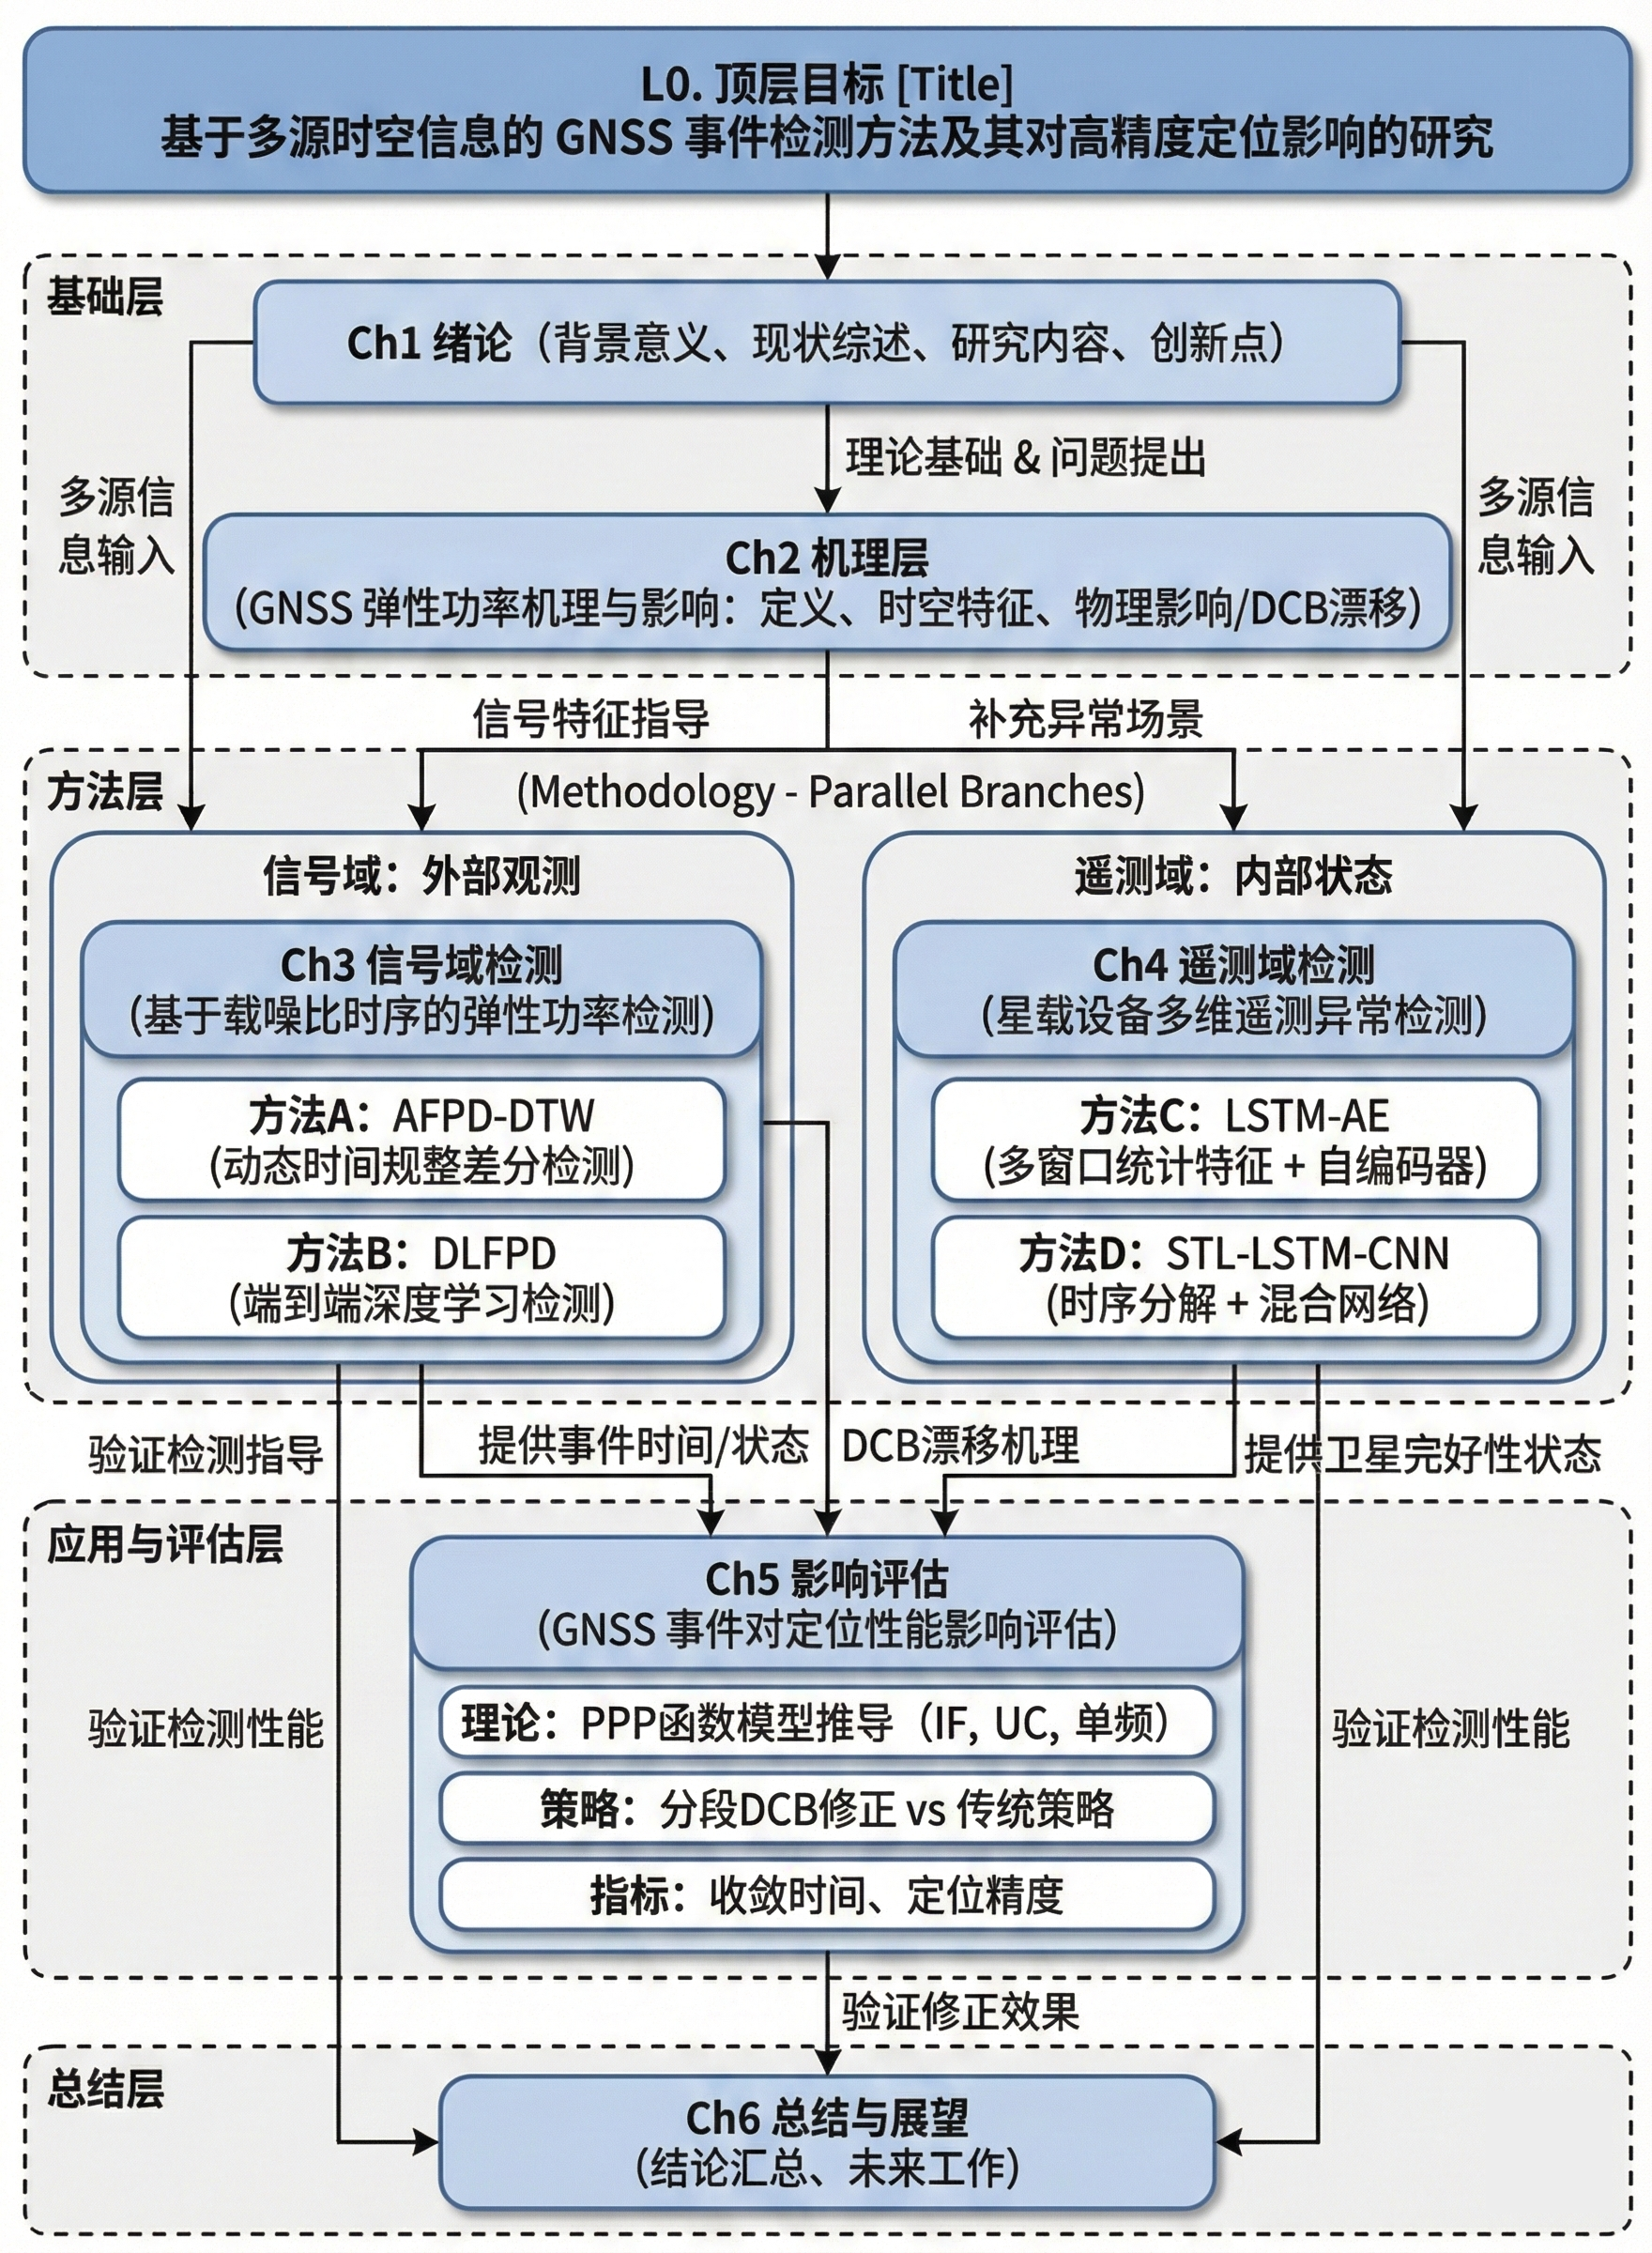
\includegraphics[width=0.85\textwidth]{c1/jiagoutu.png}
  \bicaption{本文组织架构图}{Organizational structure of this article.}
  \label{fig:c1_struct}
\end{figure}

